\documentclass[11pt]{article}

\usepackage[margin=1in]{geometry}  	% set the margins to 1in on all sides
\usepackage{graphicx}              	% to include figures
\usepackage{amsmath}               	% great math stuff
\usepackage{amsfonts}              	% for blackboard bold, etc
\usepackage{amssymb}
\usepackage{lineno}		   		   	% line numbering (see \linenumbers below)
\usepackage{setspace}		   	   	% line spacing (see \doublespacing below)
\usepackage[round]{natbib}	   	   	% referencing
\usepackage[english]{babel}
\usepackage{authblk}
\usepackage{breqn}
\usepackage[parfill]{parskip}

\begin{document}

\section*{Brief notes on possible extrapolation of ocean properties into fjords for ISMIP7}

Firstly, need to define what grid we’re provided properties on. From last time I think we used a 1 km grid extending from x=-0.72e6 to 0.96e6 and y=-3.45e6 to -0.57e6 (in metres in EPSG:3413). This gives a grid of 1680 by 2880 pixels. I’ll refer to this as the “ISMIP grid”.

Steps:

\textbf{1.} The ISMIP grid has a slightly larger extent than BedMachine. This is awkward because it means we need to extend the bed topography beyond BedMachine. To do this I used GEBCO bathymetry. The resulting extended bed topography (Fig.~\ref{extended_bathy}) has 150 m resolution inherited from BedMachine in the region covered by BedMachine, and also 150 m resolution in the extended regions, but the true resolution in the extended regions is probably coarser because they are created by interpolating from the GEBCO bathymetry, which comes on a regular 15 arc-second lat-lon grid, and I subsampled this by a factor of 5 in latitude and 20 in longitude to make the interpolation faster. We could go back and redo this at higher resolution but I don’t think it makes a big difference because the topography looks ok and this only affects regions that are far from the present day ice sheet. This extension of BedMachine is done by the extend\_bedmachine.m script and results in bedmachine\_extended.nc. The script takes about 6 minutes to run.

\begin{figure}[h!]
\centering
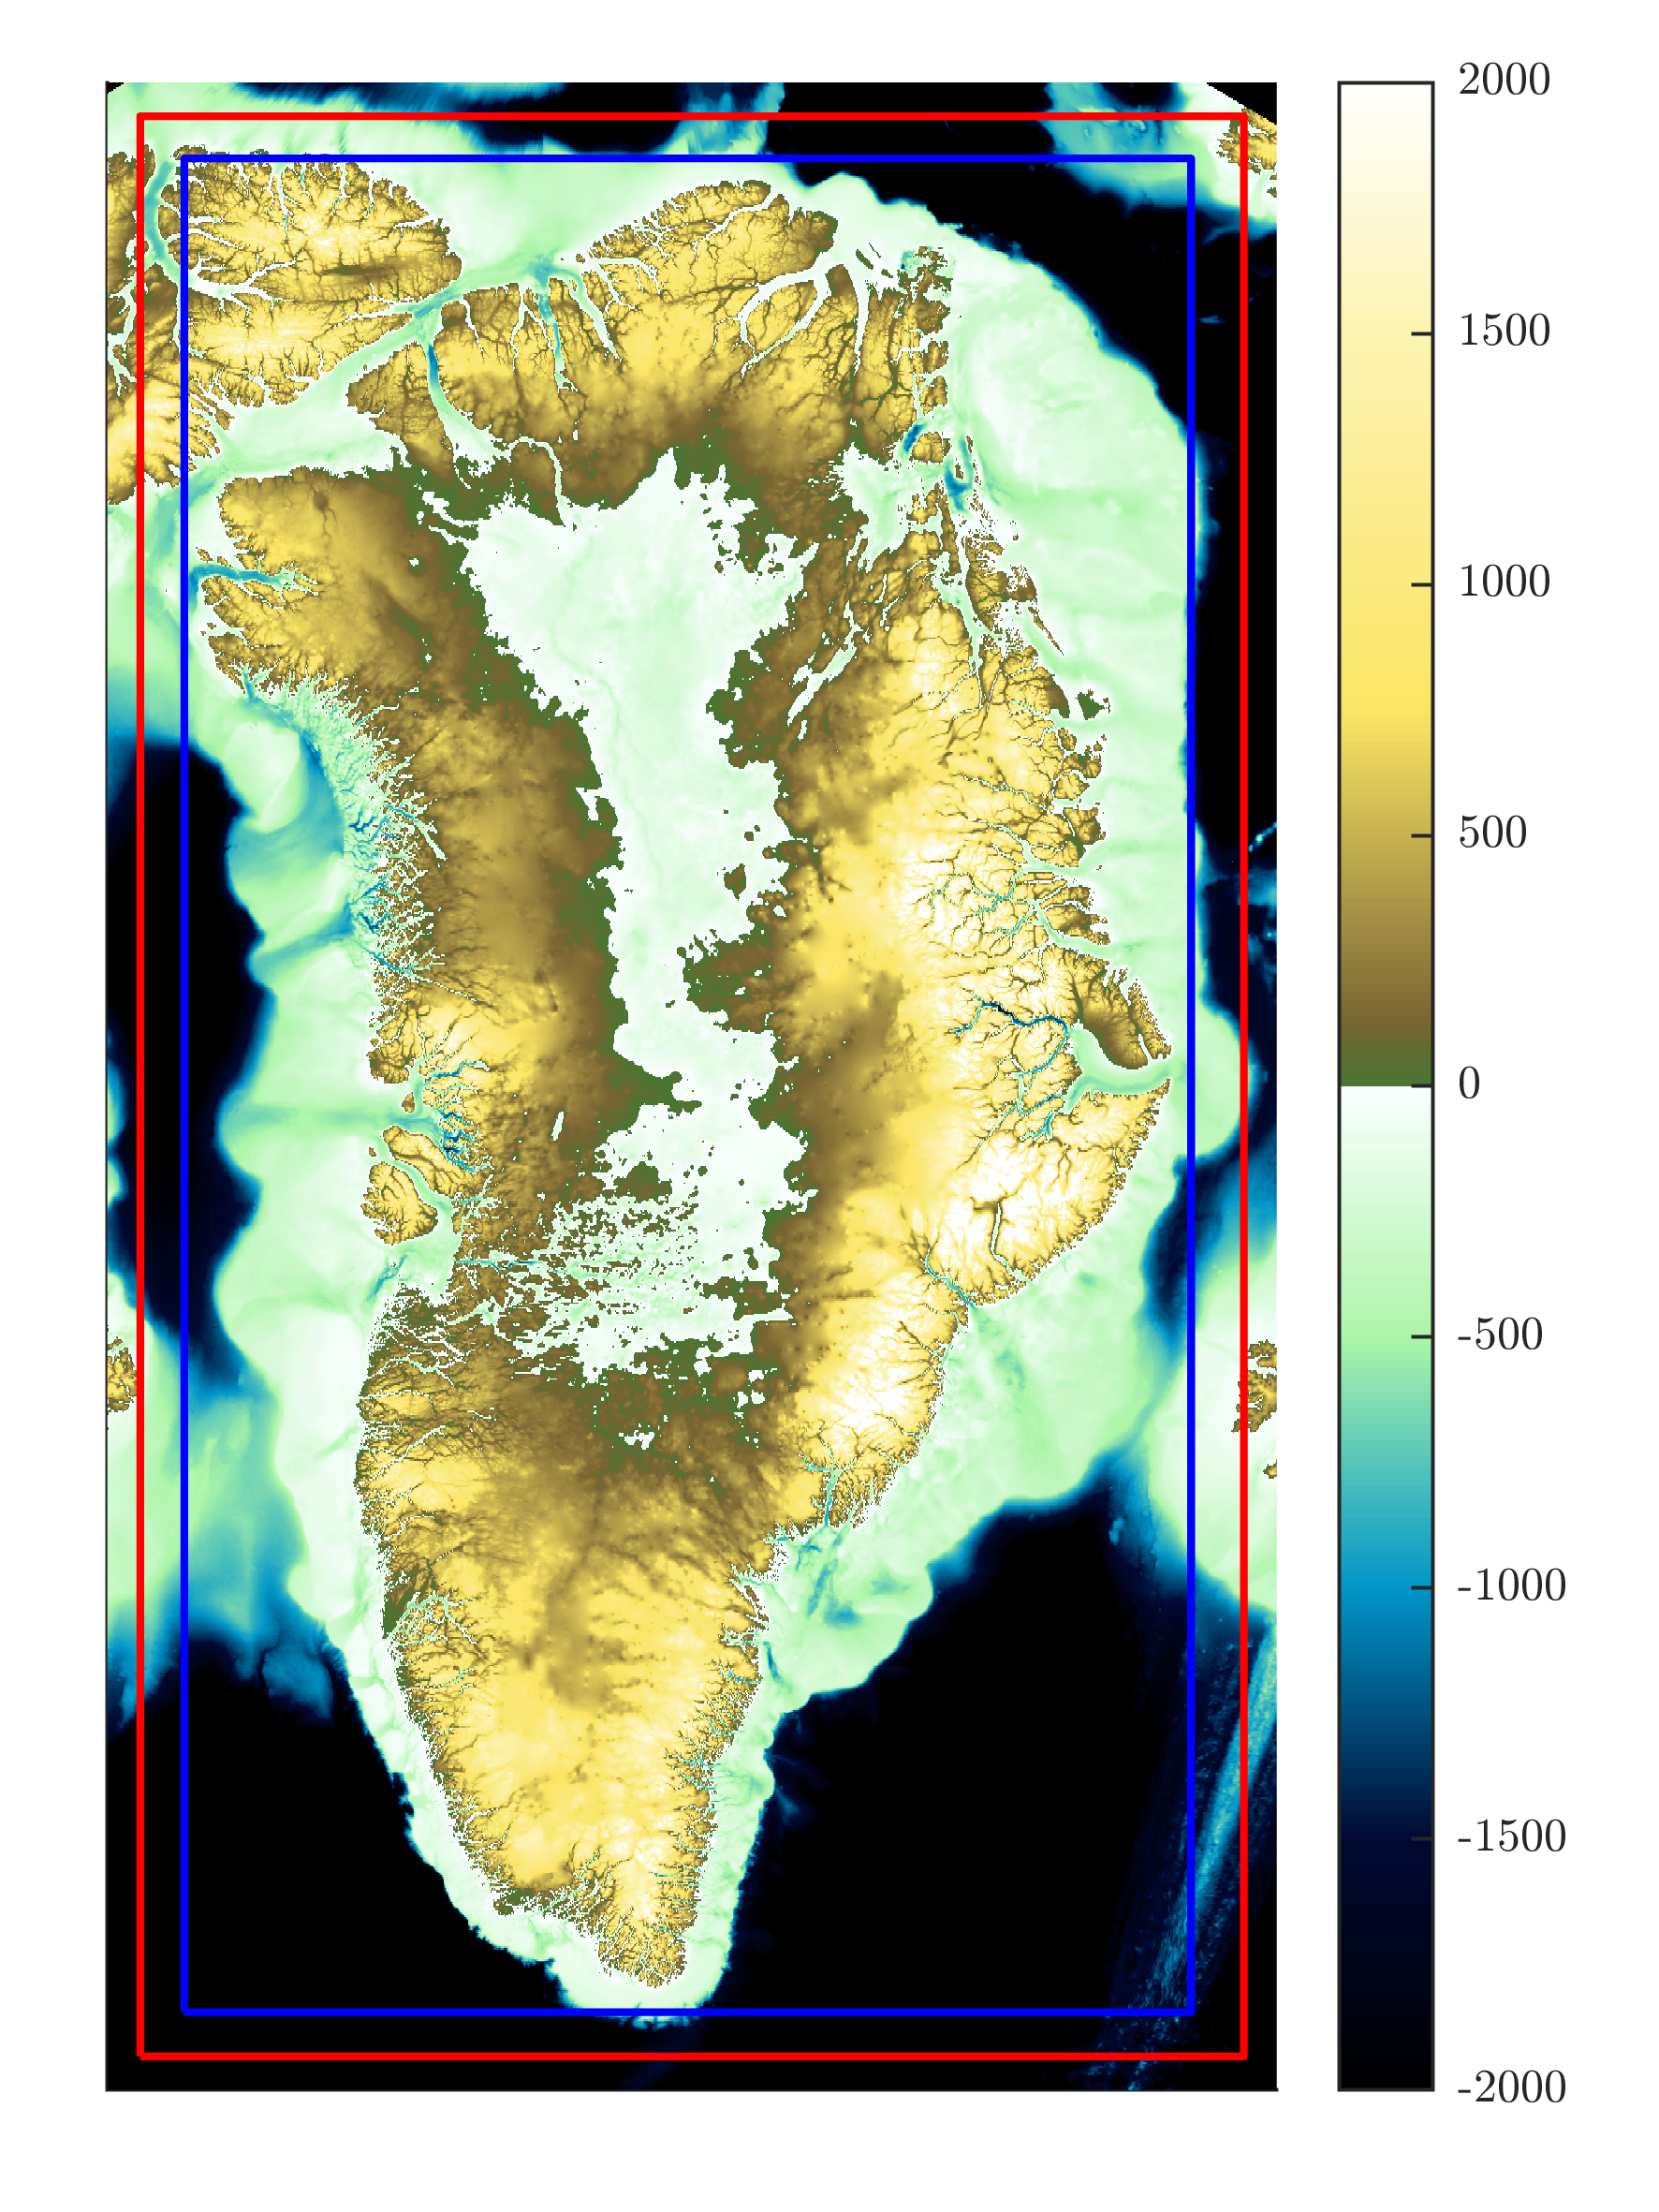
\includegraphics[width=7.5cm]{extended_bathy.png}
\caption{Extension of bathymetry. Blue outline is the extent of BedMachine, red outline is the extent of the ISMIP grid.}
\label{extended_bathy}
\end{figure}

\textbf{2.} The resulting bathymetry is slow to work with because of the high resolution. Therefore, I put the bathymetry onto the 1 km ISMIP grid by block averaging (i.e., for each 1 km square find the 150 m resolution pixels contributing to the square and take a weighted average according to how much of the pixel is in the square). The script to do this is ismip\_bed.m, which takes about 8 minutes to run, and it results in ismip\_bed.nc. From now on I work with this bed topography. We can discuss and revisit to what extent this affects the output (e.g., at 1 km, might we miss a narrow deep bit of a fjord that allows access of deep water inland? From my quick checks, I think 1 km is sufficient to capture this).

\textbf{3.} For all ISMIP grid points $(x,y)$, define the effective depth $z_{eff}(x,y)$ (Fig.~\ref{eff_depth}) as the deepest depth that has a continuous connection to a region deeper than 2000 m (i.e., the effective depth is basically the deepest depth continuously connected to an ocean basin). The depth resolution of the effective depth can be adjusted but is currently 50 m. The effective depth for above sea level points is defined as +100 m. The minimum effective depth is -2000 m; this avoids issues later on with CMIP models not having very deep points and I don't think should affect any ice sheet simulations. The effective depth for below sea level points that do not have a connection to ocean basins is assigned NaN – this applies to a few regions below the present day ice sheet where the bed is below sea level and there is no connection to the outside ocean. The script for this is effective\_depth.m, takes just seconds to run, and results in z\_eff.nc.

\begin{figure}[h!]
\centering
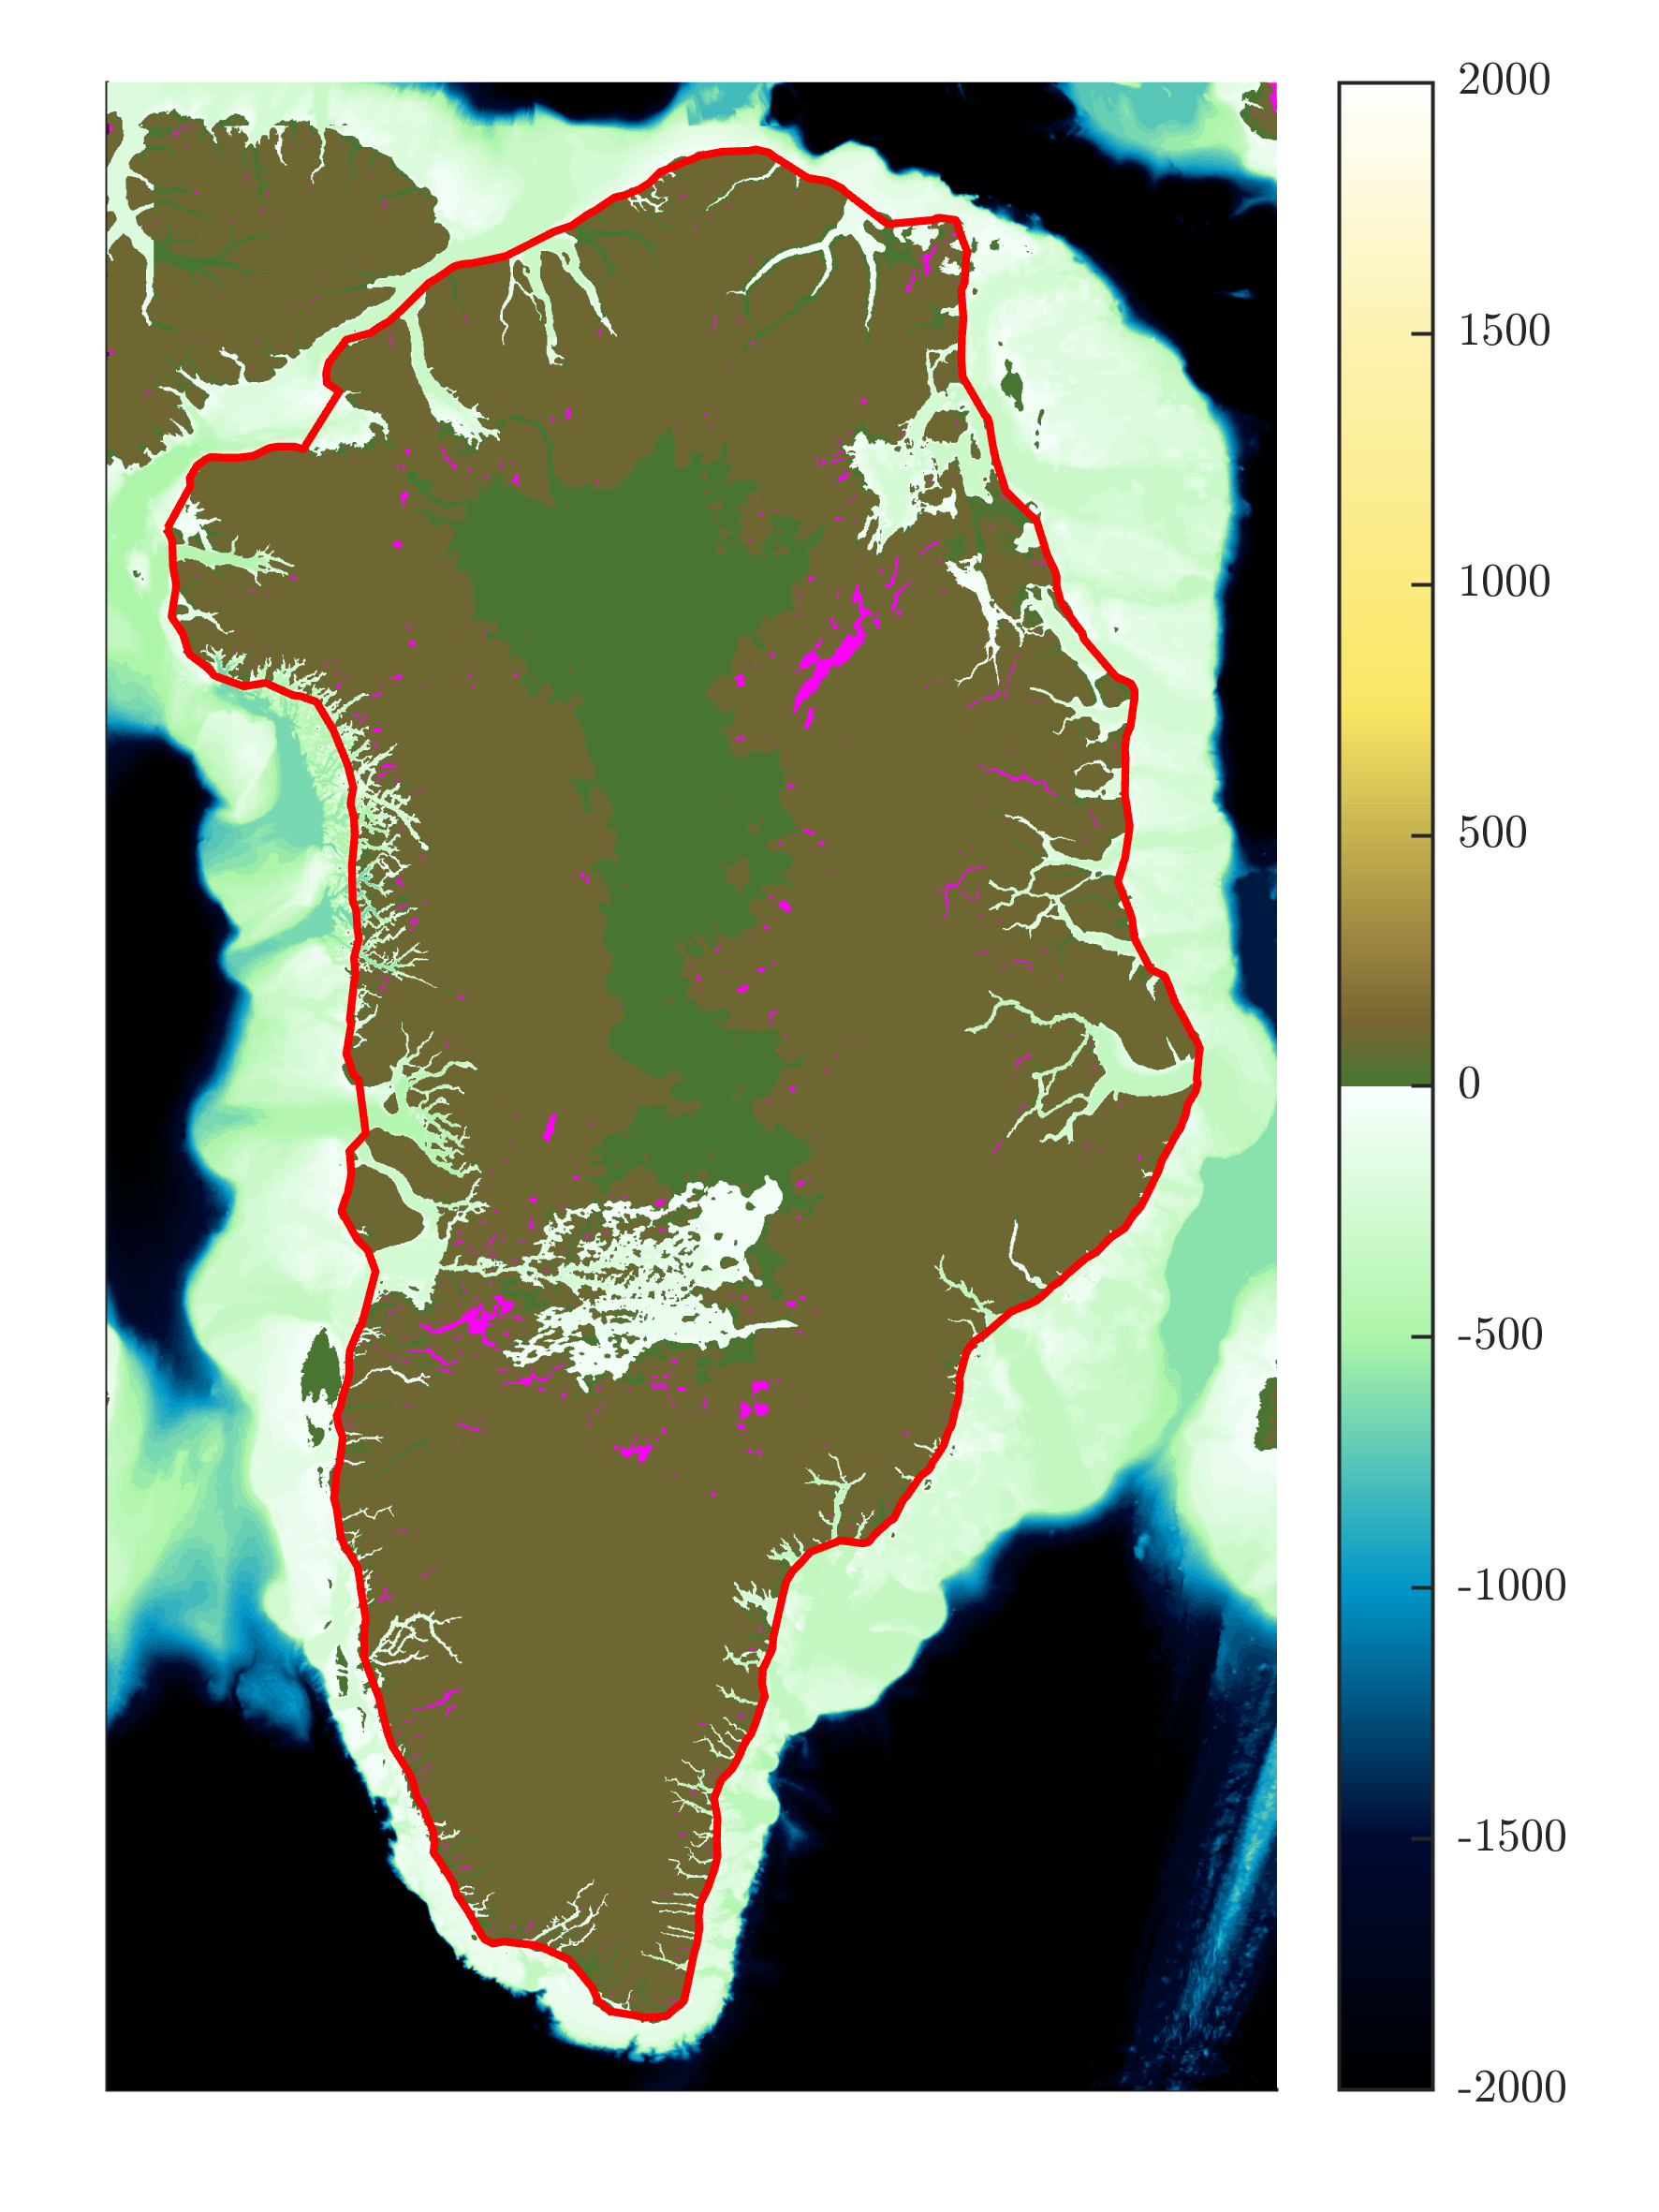
\includegraphics[width=7.5cm]{effective_depth.png}
\caption{Effective depth. Note magenta regions which are below sea level but not connected to the ocean. The red line is the convex hull.}
\label{eff_depth}
\end{figure}

\textbf{4.} Define the convex hull of Greenland (imagine stretching a rubber band around Greenland then letting it contract) - see Fig.~\ref{eff_depth}. We use this to separate the forcing grid into a region outside the convex hull (which is generally resolved by CMIP models) and a region inside the convex hull. These are then treated differently in the next step. The convex hull is done by the script shrinkwrap\_greenland.m, takes less than a minute and results in fjord\_shelf\_boundary.csv.

\textbf{5.} For all wet points $(x,y)$ that have an open connection to the ocean (i.e., all points with an effective depth of 0 or less), we now define an effective position $[X_{eff}(x,y), Y_{eff}(x,y)]$. The idea is that the effective position will be close to the place where ocean waters for that point will be sourced from. For points outside the convex hull, the effective position is the same as the actual position (i.e., ocean properties at that point are likely to come from the CMIP model at that point). For points inside the convex hull, the effective position is the nearest point outside the hull connected by a continuous wet path. This is best explained by visualisation (Fig.~\ref{eff_pos}). The script to do this is effective\_position.m and it takes about 10 minutes to run, and produces XY\_eff.nc.

\begin{figure}[h!]
\centering
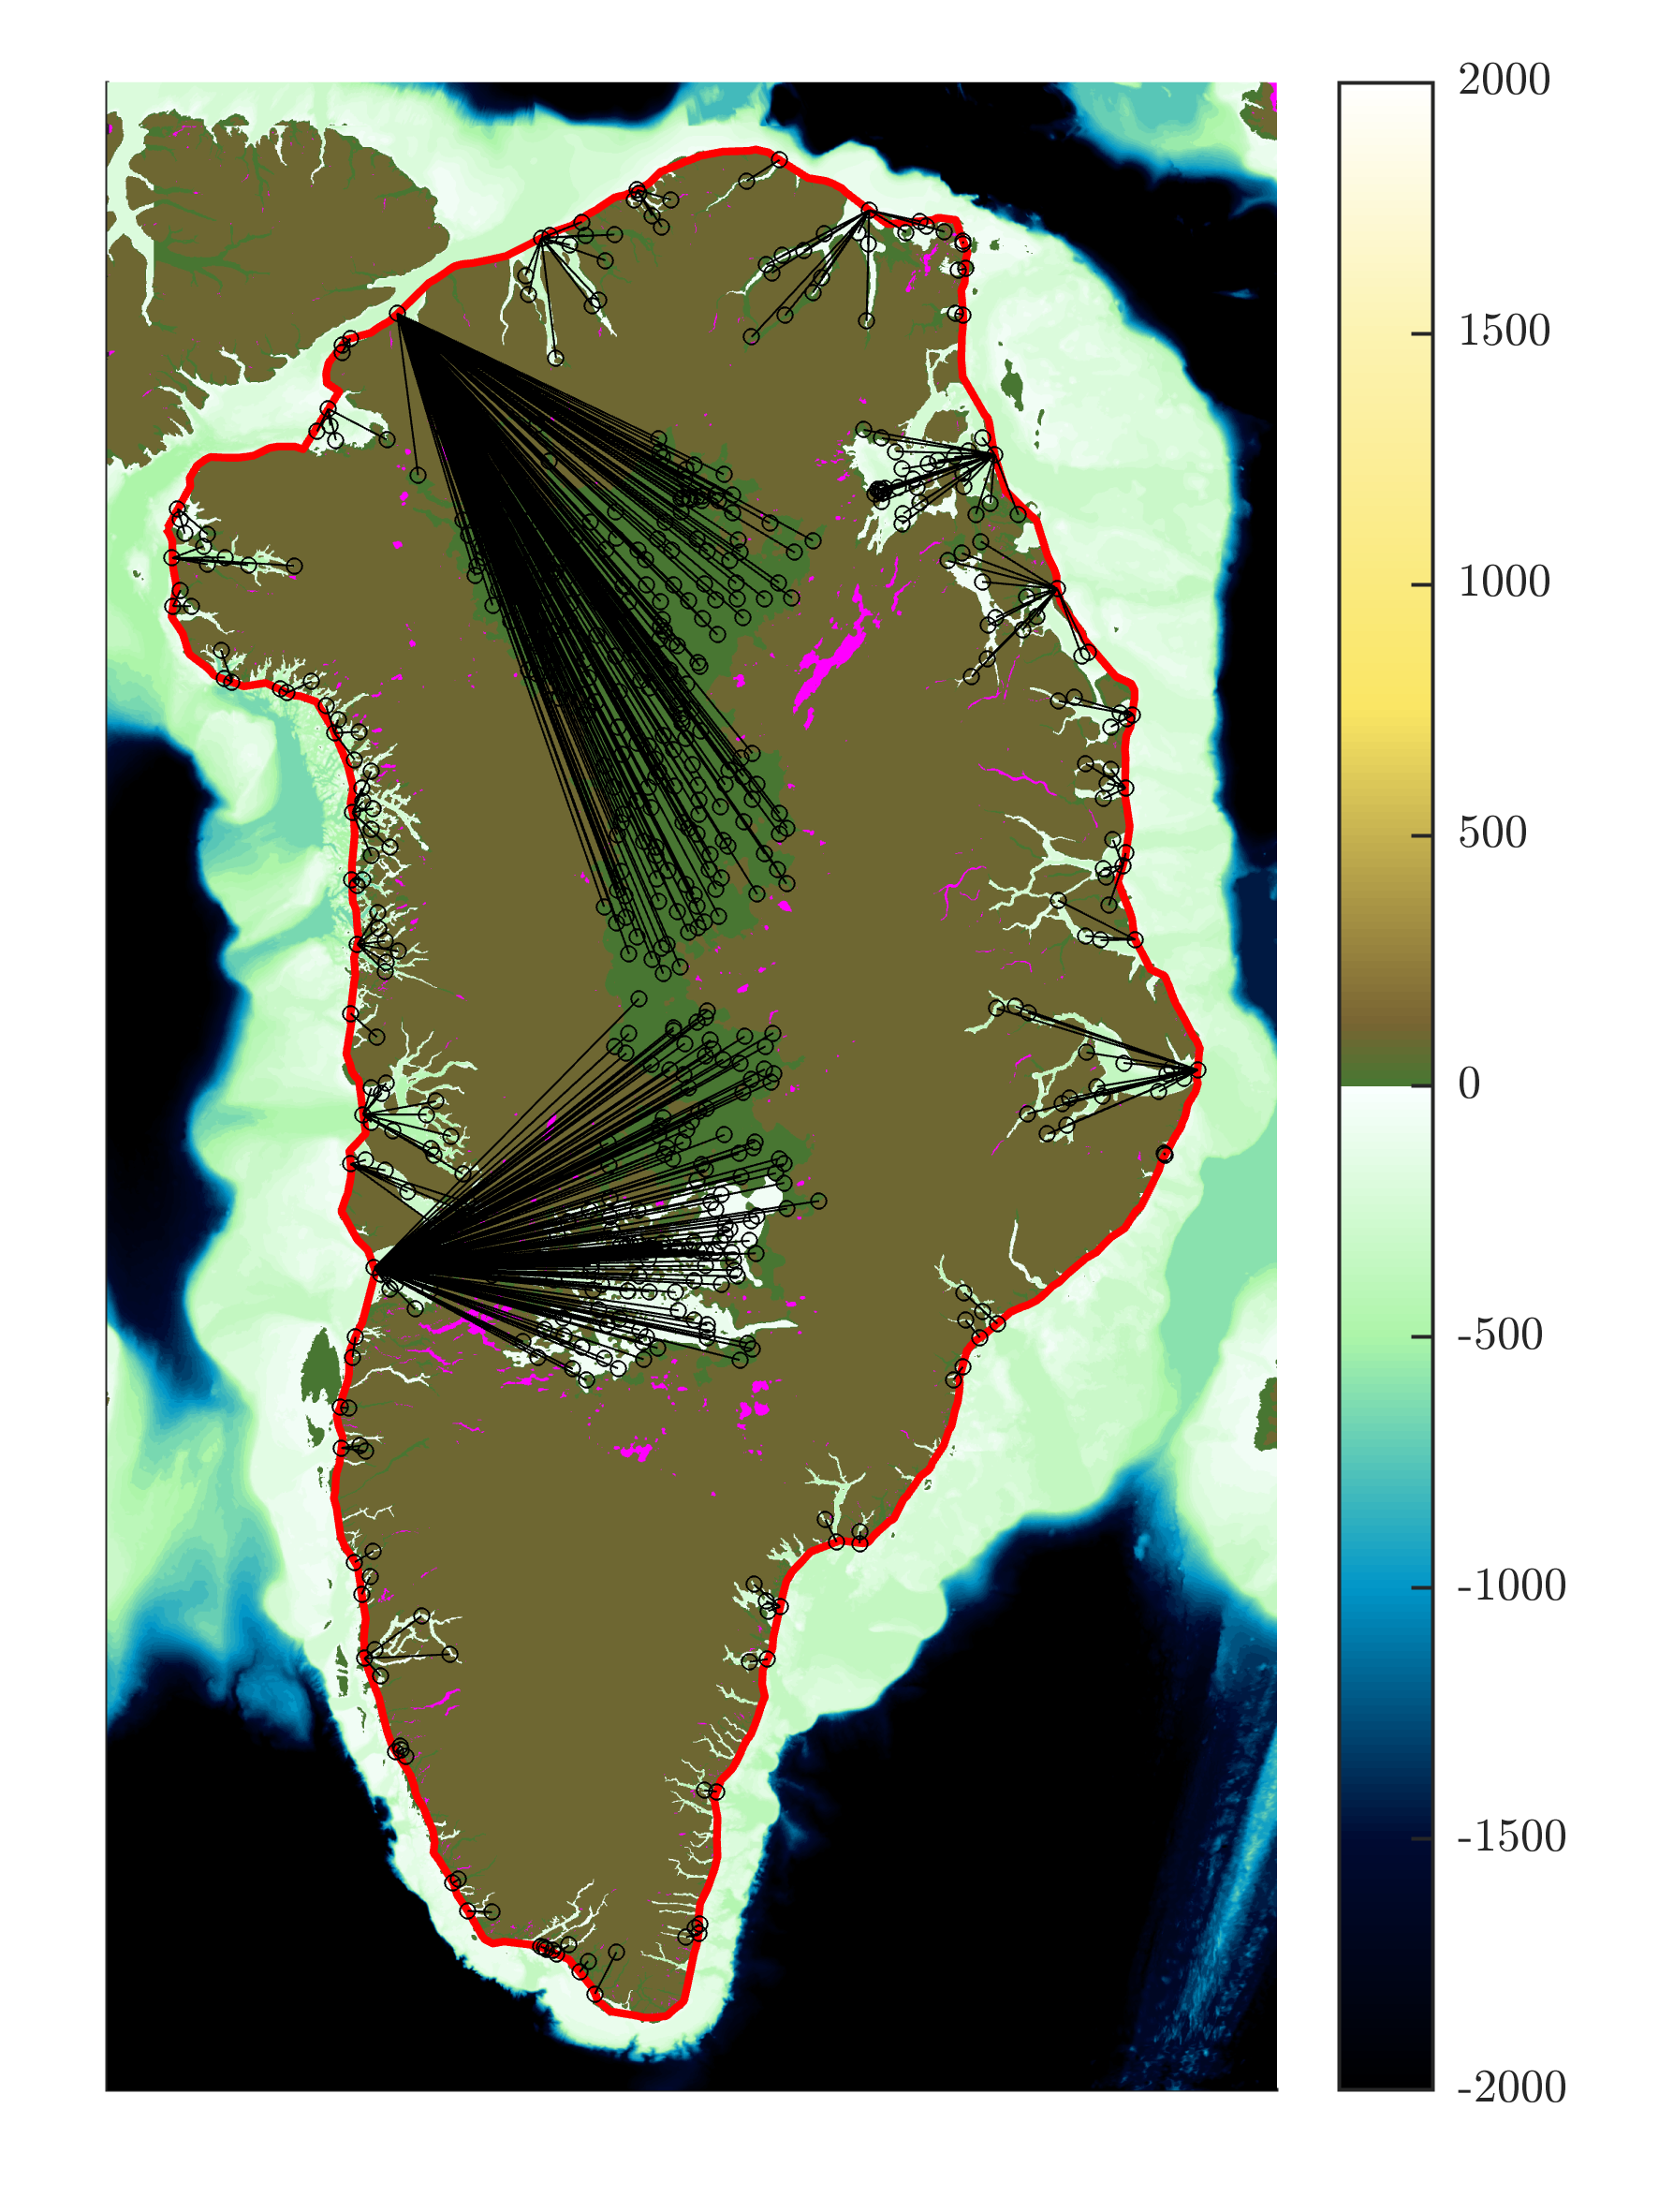
\includegraphics[width=7.5cm]{effective_positions.png}
\caption{Effective positions, only shown for a subset of the points inside the convex hull (points outside the convex hull just map to themselves). On the plot, each line connects two points - one point is $(x,y)$ and is inside the convex hull, and the other point is $[X_{eff}(x,y), Y_{eff}(x,y)]$ and is outside the convex hull.}
\label{eff_pos}
\end{figure}

At this point, the idea is that for each wet point $(x,y)$ with a connection to the ocean, we have an effective position $[X_{eff}(x,y), Y_{eff}(x,y)]$ which is the position where ocean waters are sourced from (e.g., Fig.~\ref{eff_pos}), and we have an effective depth $z_{eff}(x,y)$ which is the depth at which we’ll sample the ocean waters (Fig.~\ref{eff_depth}). We only have to do this once, rather than individually for each CMIP model. The part that’s left is matching up the CMIP model points to the effective positions and depths.

Now, given CMIP model output we do the following (example is for MIROC6, ssp585, r1i1p1f1 and I only show one time snapshot). This is all done by script associate\_properties.m and it takes less than a minute.

\textbf{6.} Calculate CMIP thermal forcing on the same vertical grid as the effective depths were calculated on, but do this assuming the thermal forcing applies at the surface (we'll apply the depth/pressure correction later). Call this $\text{TF}_{nop}(i,z,t)$, given by $\text{TF}_{nop}(i,z,t)=T(i,z,t)-\left[\lambda_1S(i,z,t)+\lambda_2\right]$ using the usual linearised freezing point, and where $T$ and $S$ are temperature and salinity. Note that the $i$ is a linear spatial index because the CMIP points are not on a regular grid.

\textbf{7.} Calculate the depth $z_{cmip}$ of the CMIP model points as the deepest depth at each point at which we have a value of $\text{TF}_{nop}(i,z,t)$. See Fig.~\ref{cmip_depth}.

\begin{figure}[h!]
\centering
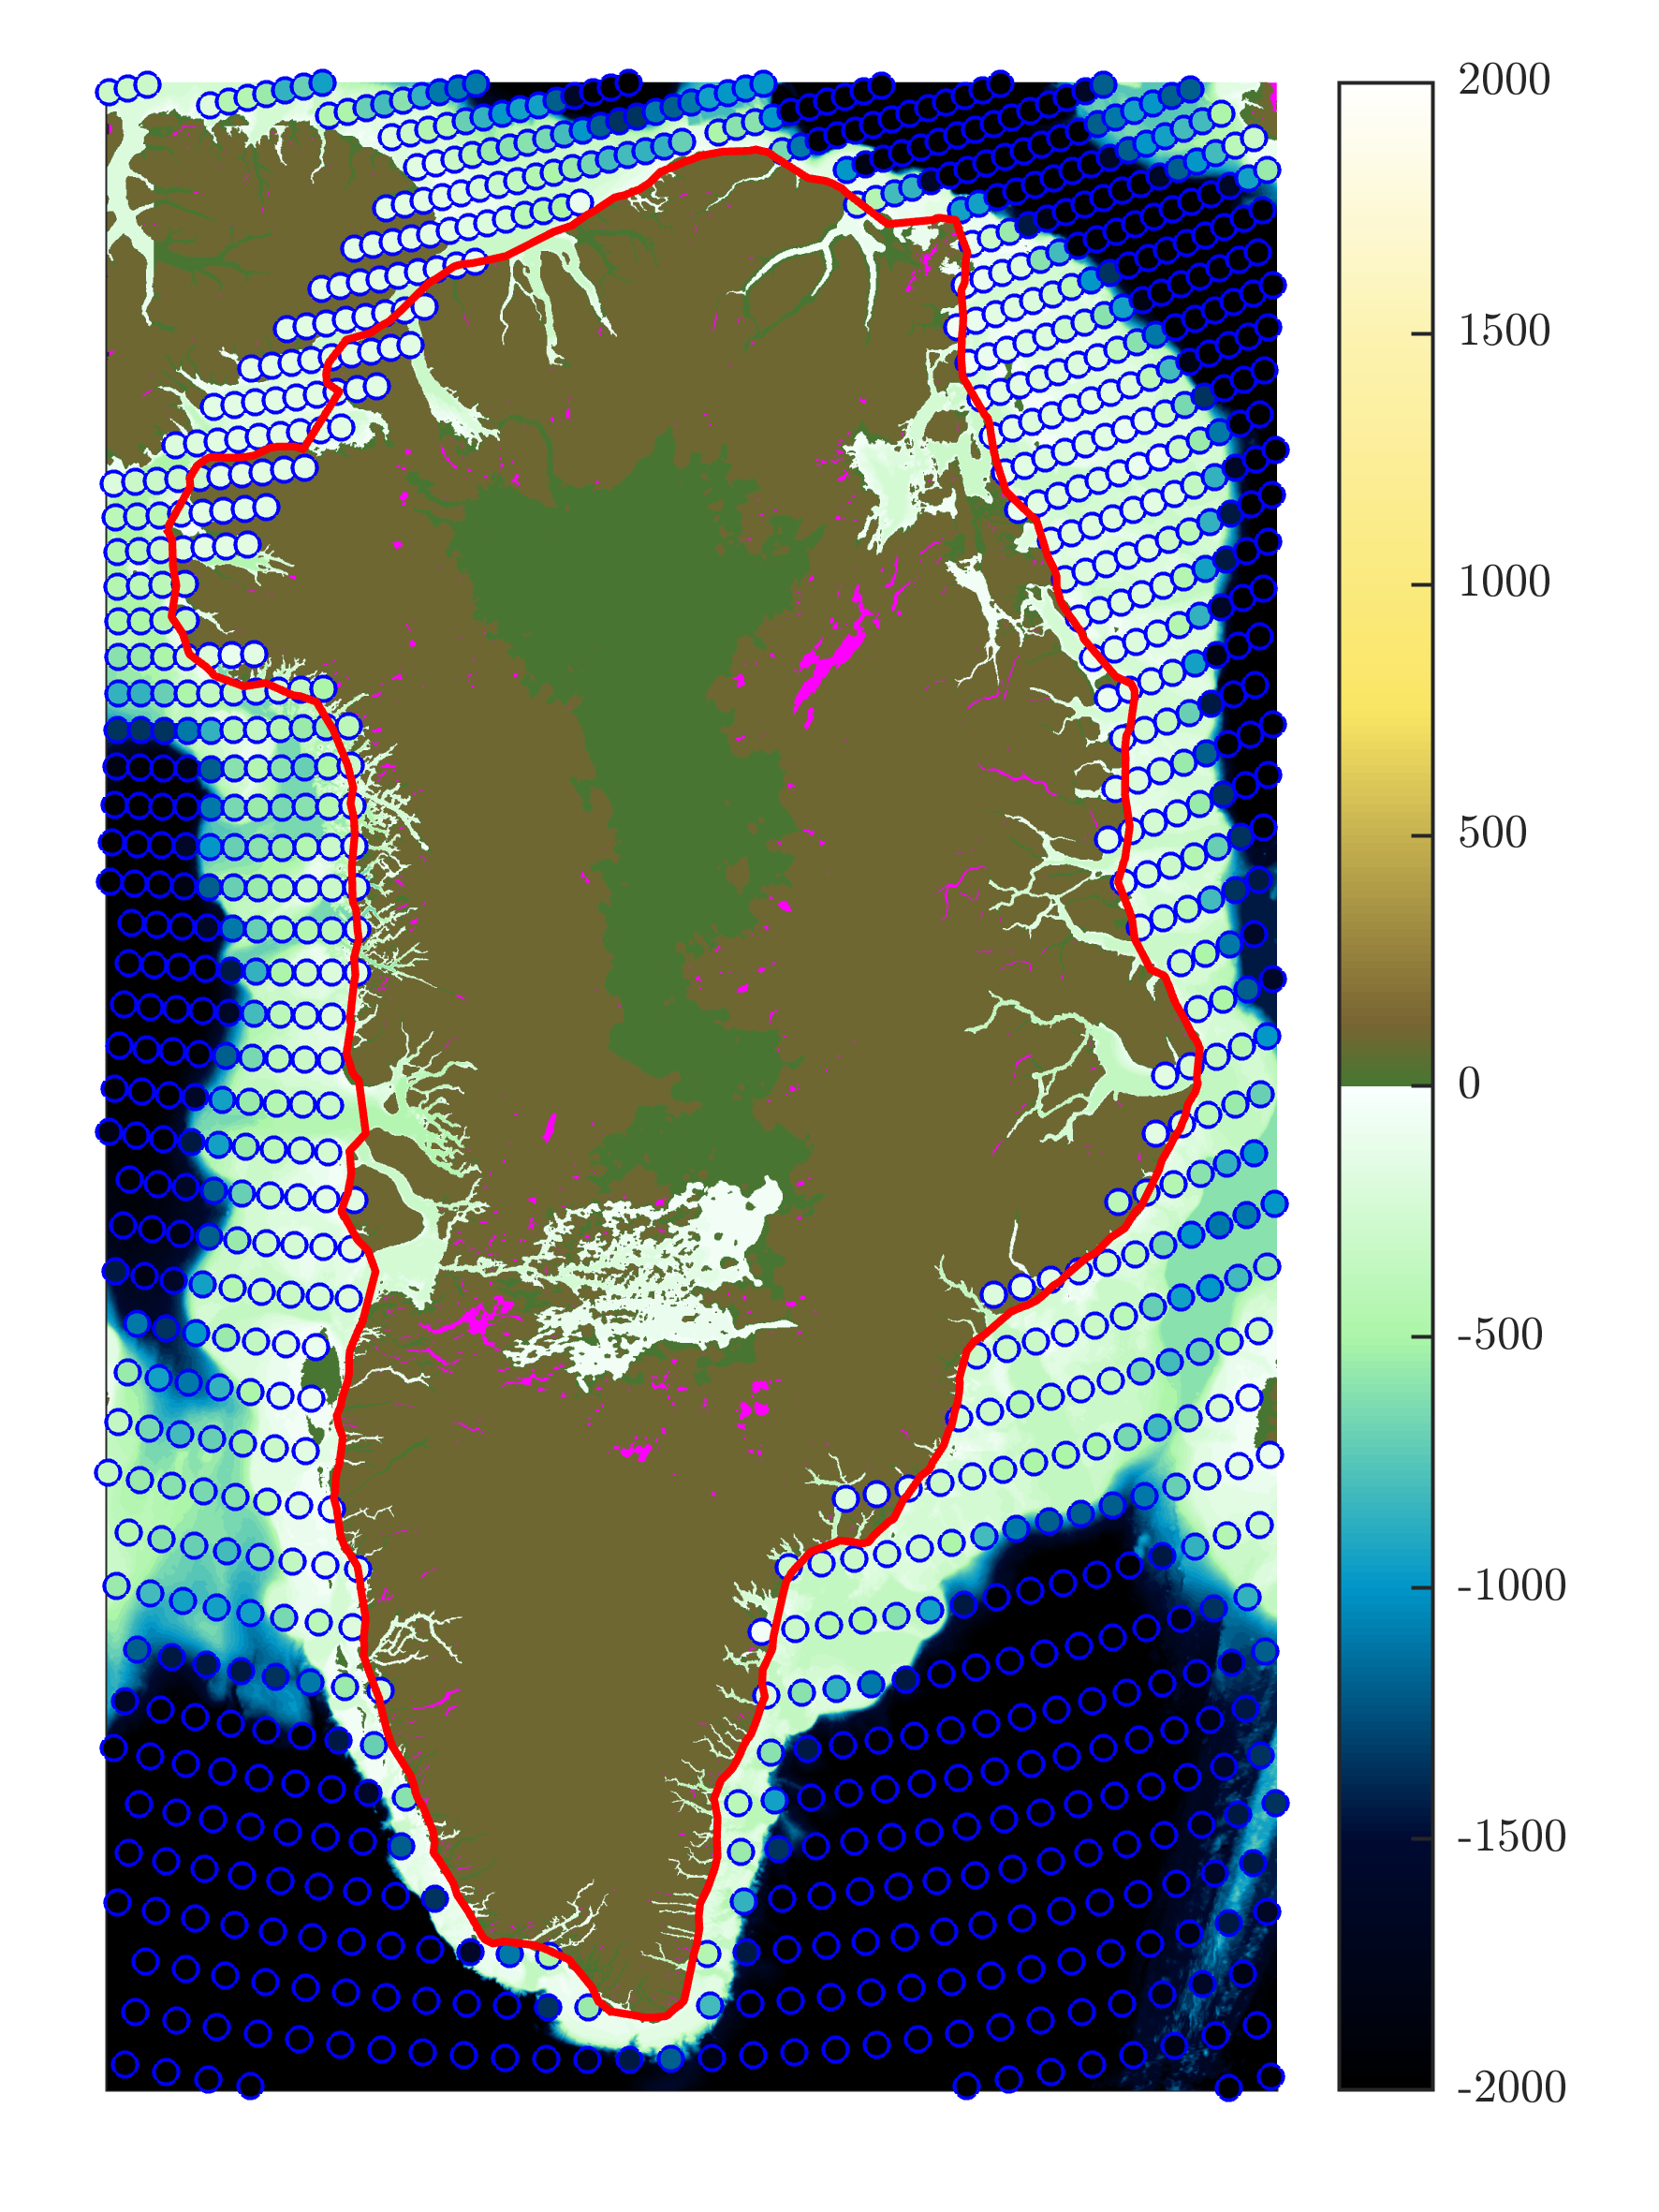
\includegraphics[width=7.5cm]{cmip_depth.png}
\caption{MIROC6 model points and depths (coloured markers), overlaid on ISMIP effective depths.}
\label{cmip_depth}
\end{figure}

\textbf{8.} For all wet points $(x,y)$ connected to the ocean find the CMIP grid point closest to $[X_{eff}(x,y), Y_{eff}(x,y)]$ satisfying $z_{cmip}<z_{eff}(x,y)$. In other words, for each point that is connected to the ocean, we find the CMIP grid point that has properties sufficiently deep and is closest to the effective position. Save the index $\tilde{i}(x,y)$ of this point (i.e., $\tilde{i}$ tells us the CMIP grid point we will sample from). Note that there are a few different things that could happen here: (i) $(x,y)$ is inside the convex hull and there is a CMIP point on the shelf with enough depth close to $[X_{eff}(x,y), Y_{eff}(x,y)]$ - we take properties from that CMIP point; (ii) $(x,y)$ is inside the convex hull but there are no points on the shelf close to $[X_{eff}(x,y), Y_{eff}(x,y)]$ that are deep enough, so we end up selecting a nearby point just off the shelf; (iii) $(x,y)$ is outside the convex hull on the shelf and is close to a CMIP point with deep enough properties - we use those; (iv) $(x,y)$ is outside the convex hull on the shelf but we have to go off the shelf to find a CMIP point with deep enough properties. With more time I could probably find examples of these and add them to Fig.~\ref{cmip_depth}. In this way we are accounting not only for the fact that the CMIP models don't resolve fjords but also for the fact that they might have too shallow bathymetry on the shelf.

\textbf{9.} Define the thermal forcing for each wet point $(x,y)$ connected to the ocean as $\text{TF}_{nop}(x,y,t)=\text{TF}_{nop}(\tilde{i}(x,y),z_{eff}(x,y),t)$. That is, we take the properties from the selected CMIP point at the effective depth. Finally, we correct the thermal forcing for the effective depth, using $\text{TF}(x,y,t)=\text{TF}_{nop}(x,y,t)+\lambda_3z_{eff}(x,y)$. Our final result is $\text{TF}(x,y,t)$ (Fig.~\ref{T_example}). Note that we check for any values where $\text{TF}<0$ and reset these to 0. We also assign $\text{TF}=0$ to all points that are below sea level but not connected to the ocean (e.g., Fig.~\ref{eff_depth}, magenta).

\begin{figure}[h!]
\centering
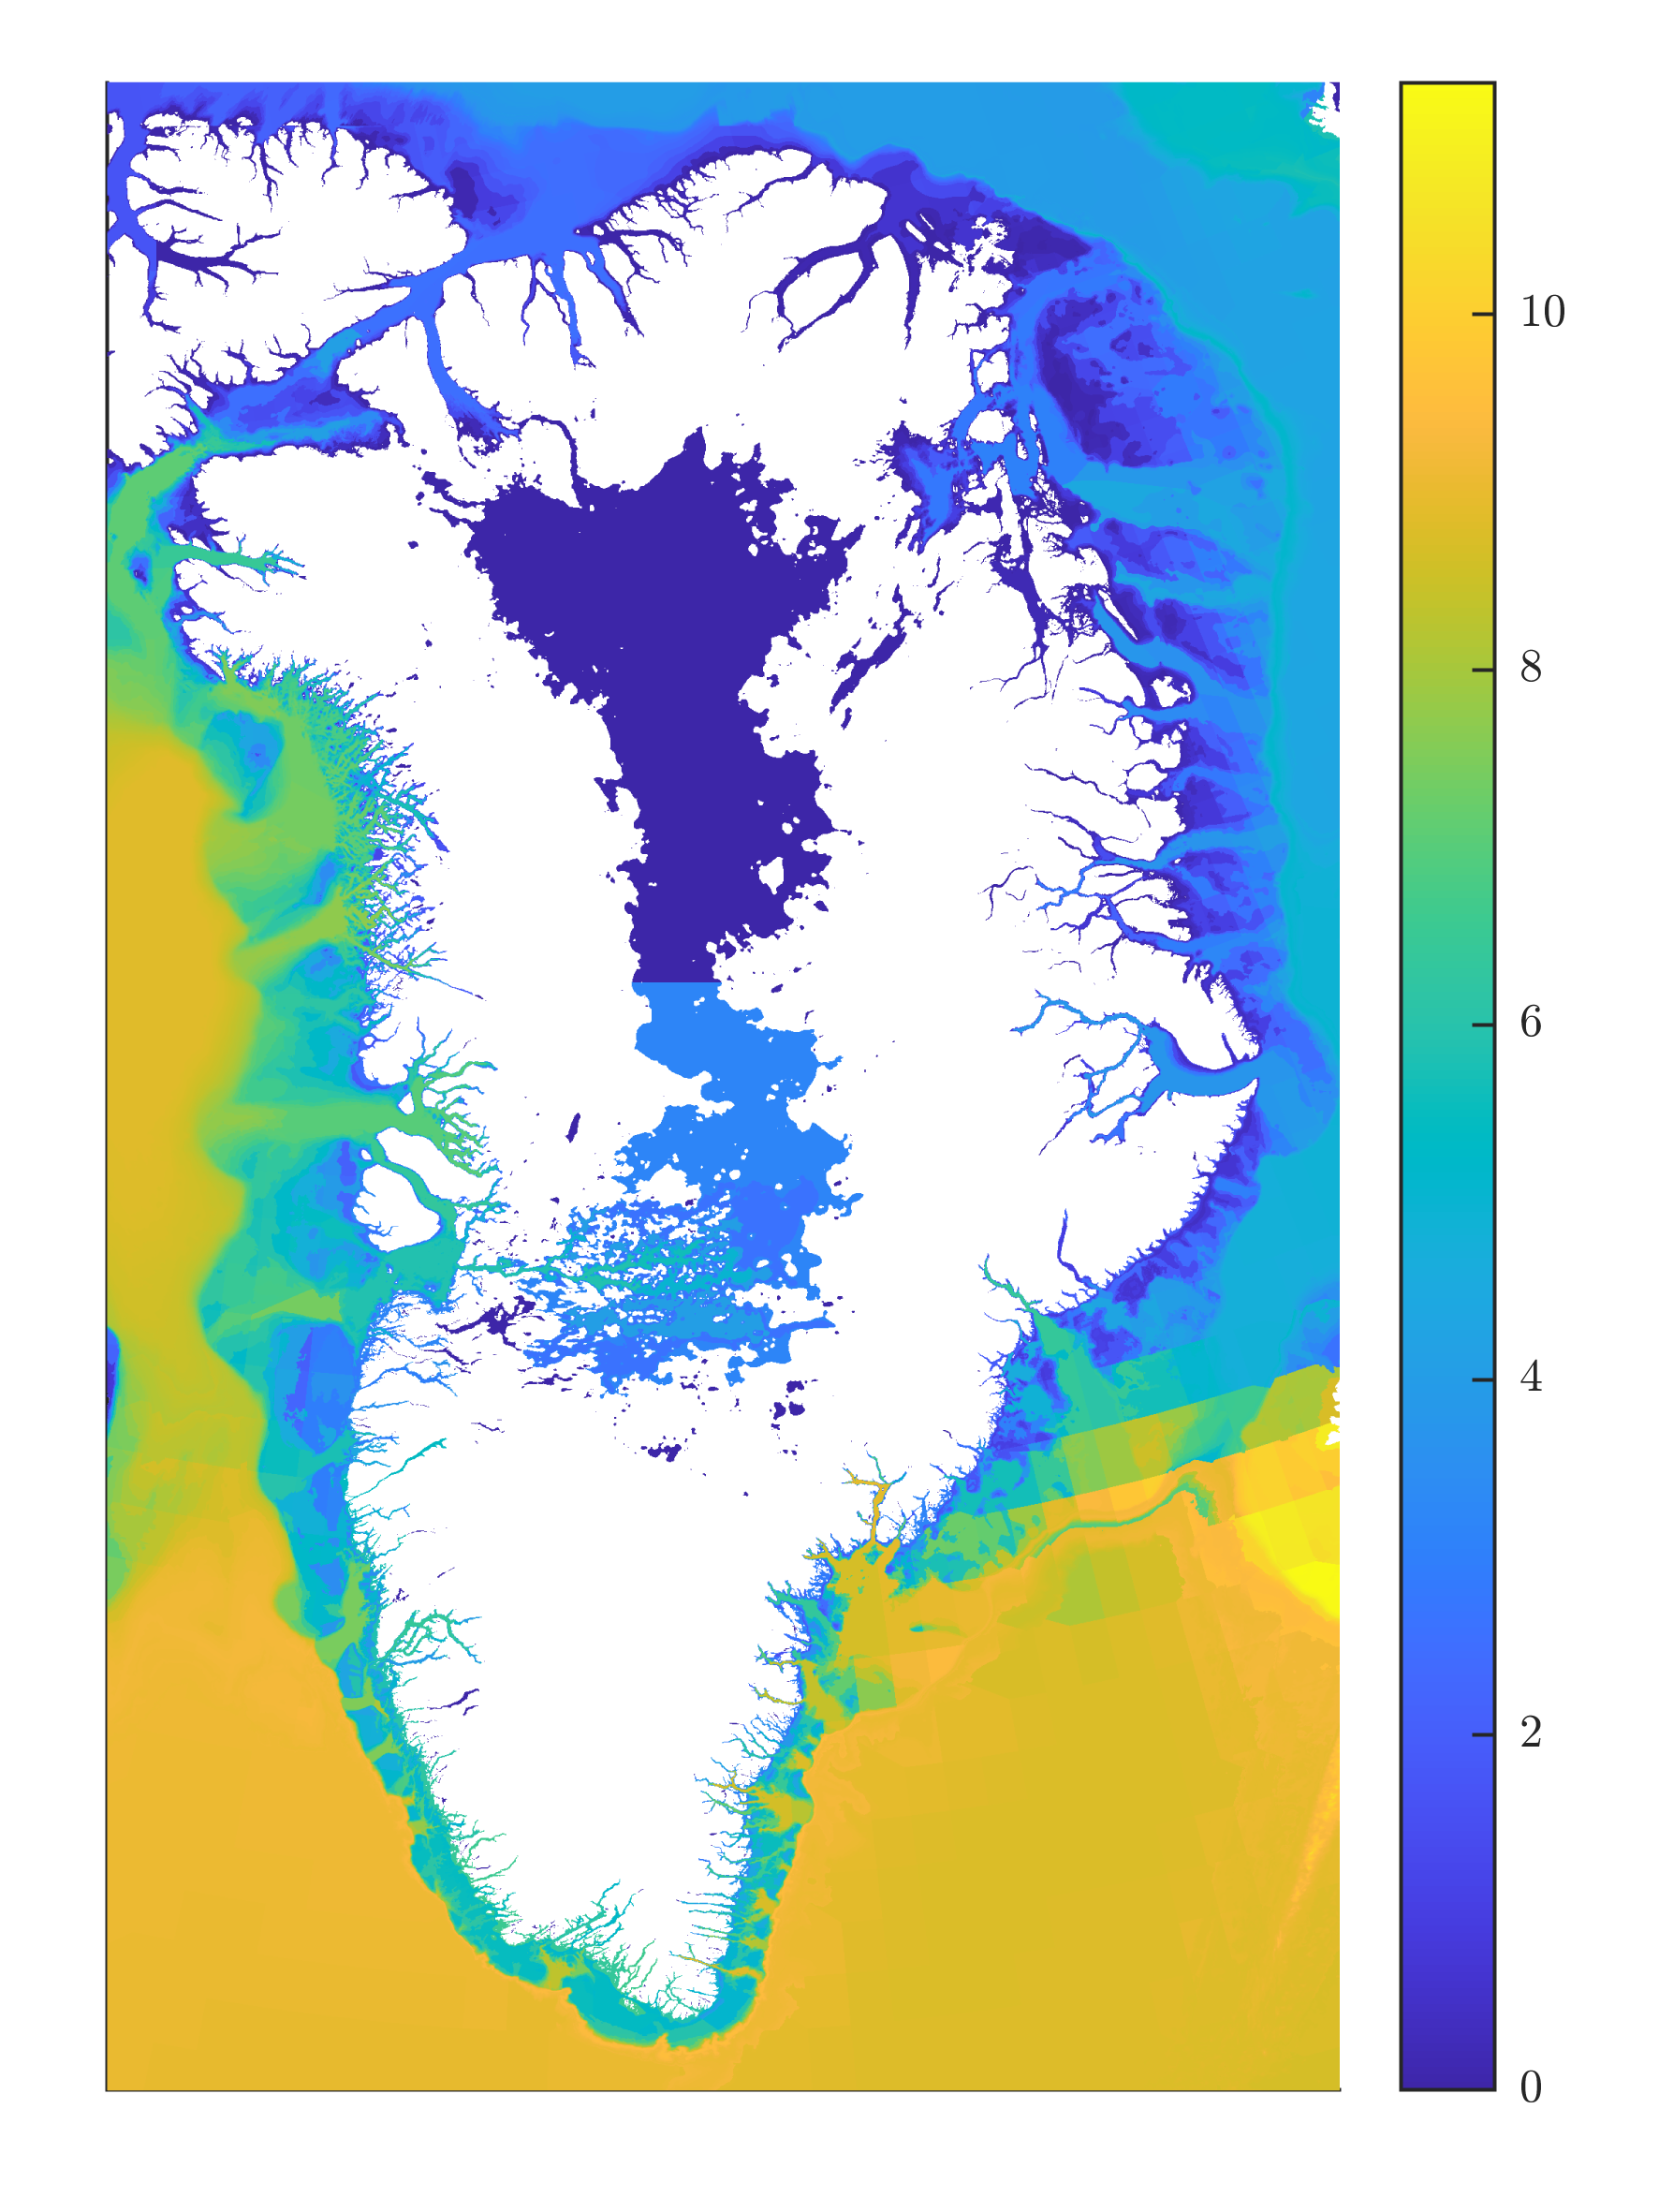
\includegraphics[width=7.5cm]{TF_example.png}
\caption{Example of final thermal forcing $\text{TF}(x,y,t)$ for a time snapshot of the MIROC6, ssp585 simulation.}
\label{T_example}
\end{figure}


\end{document}